\documentclass{beamer}

\usepackage[utf8]{inputenc}
\usepackage{hyperref}

\usetheme{Berkeley}
\beamertemplatenavigationsymbolsempty
\setbeamertemplate{headline}{}
 
\title{Geo-Clustering in FoodChain-Lab}
\date{}
 
\begin{document}
\maketitle

\section{ }

\subsection{Tasks}
\begin{frame}
	\begin{itemize}
		\item Perform a clustering using the following workflow: \url{https://github.com/SiLeBAT/BfROpenLabResources/raw/master/GitHubPages/workflows/FCL_Example.zip}
		\item Cluster all French primary producers by using the \textbf{GIS Cluster} node.
		\item Use a \textbf{Max Neighborhood Distance} of 100km.
		\item That means two stations are put into the same cluster if their distance is less than 100km.
	\end{itemize}
\end{frame}
 
\subsection{1}
\begin{frame}
	\begin{center}
  		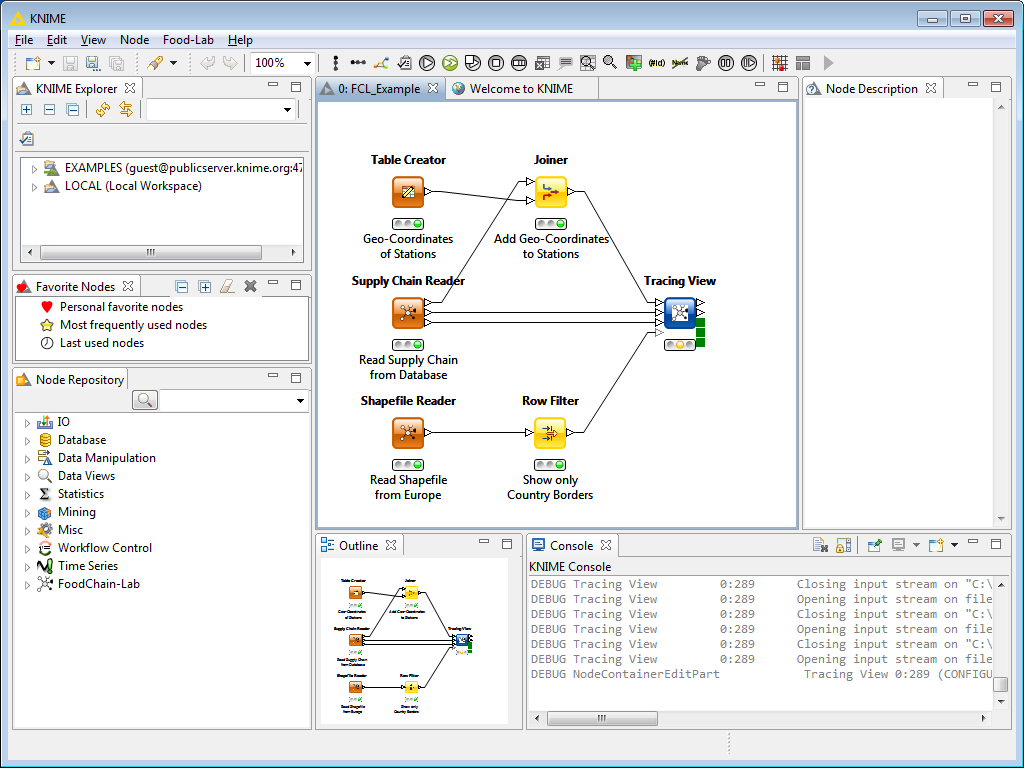
\includegraphics[height=0.6\textheight]{1.png}
	\end{center}
	\begin{itemize}
		\item Import the Example Workflow from \url{https://github.com/SiLeBAT/BfROpenLabResources/raw/master/GitHubPages/workflows/FCL_Example.zip}.
	\end{itemize}
\end{frame}

\subsection{2}
\begin{frame}
	\begin{center}
  		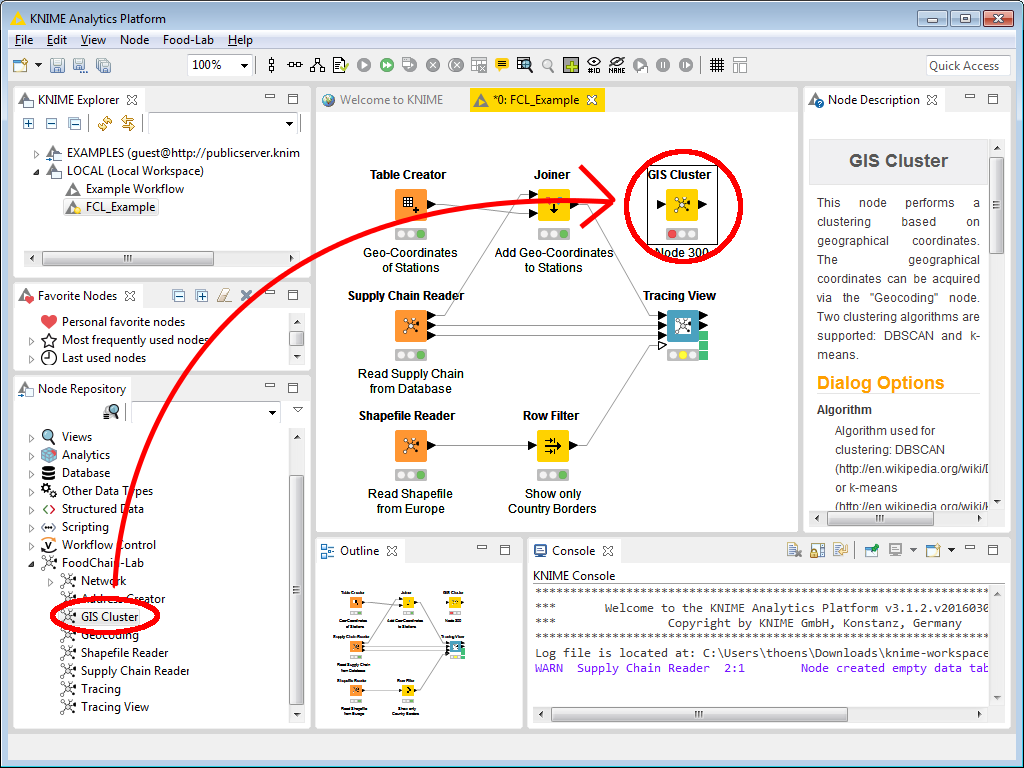
\includegraphics[height=0.6\textheight]{2.png}
	\end{center}
	\begin{itemize}
		\item Drag the \textbf{GIS Cluster} node from \textbf{FoodChain-Lab} in the \textbf{Node Repository} to the \textbf{Workflow Editor}.
	\end{itemize}
\end{frame}

\subsection{3}
\begin{frame}
	\begin{center}
  		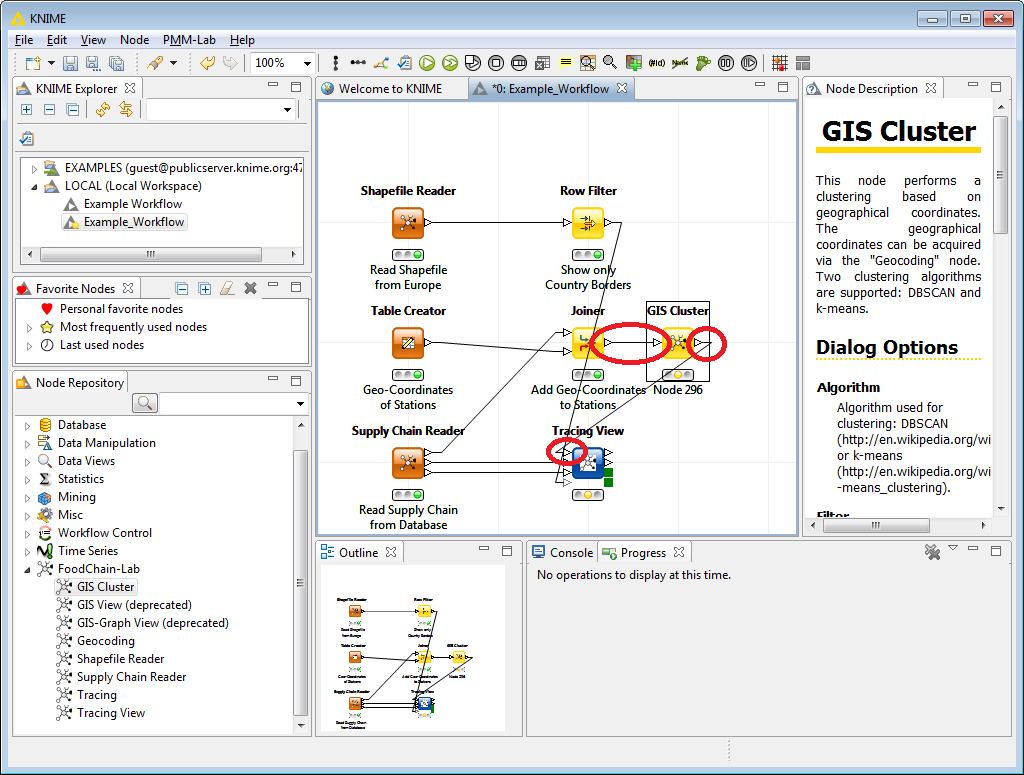
\includegraphics[height=0.6\textheight]{3.png}
	\end{center}
	\begin{itemize}
		\item Connect the output of \textbf{Joiner} to the input of \textbf{GIS Cluster}.
		\item Connect the output of \textbf{GIS Cluster} to the first input of \textbf{Tracing View}.
		\item Double click on the \textbf{GIS Cluster} node to open its dialog.
	\end{itemize}
\end{frame}

\subsection{4}
\begin{frame}
	\begin{center}
  		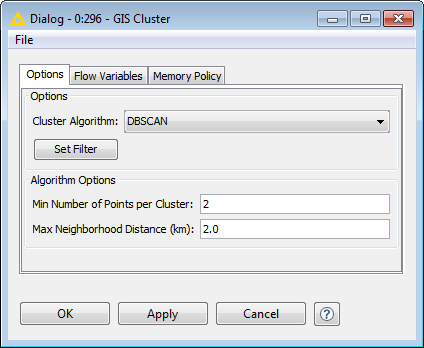
\includegraphics[height=0.6\textheight]{4.png}
	\end{center}
	\begin{itemize}
		\item In this dialog you can set up an algorithm for geographical clustering based on latitude and longitude.
		\item Click on \textbf{Set Filter} to define which stations should be clustered.
	\end{itemize}
\end{frame}

\subsection{5}
\begin{frame}
	\begin{center}
  		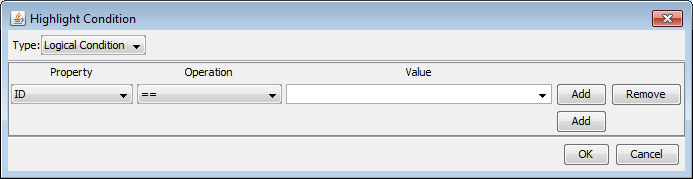
\includegraphics[width=0.9\textwidth]{5.png}
	\end{center}
	\begin{itemize}
		\item You should see this dialog now.
		\item Press the button in the red circle to change the \textbf{Property} value.
	\end{itemize}
\end{frame}

\subsection{6}
\begin{frame}
	\begin{center}
  		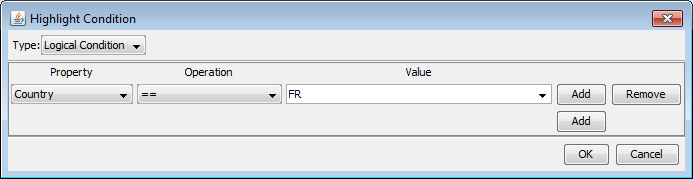
\includegraphics[width=0.7\textwidth]{6.png}
	\end{center}
	\begin{itemize}
		\item Select "Country".
	\end{itemize}
\end{frame}

\subsection{7}
\begin{frame}
	\begin{center}
  		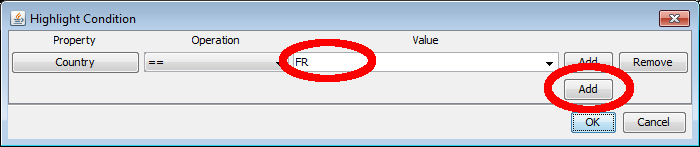
\includegraphics[width=0.9\textwidth]{7.png}
	\end{center}
	\begin{itemize}
		\item Now select "FR" as \textbf{Value}, since we want to cluster stations in France.
		\item Afterwards press \textbf{Add} to add another condition.
	\end{itemize}
\end{frame}

\subsection{8}
\begin{frame}
	\begin{center}
  		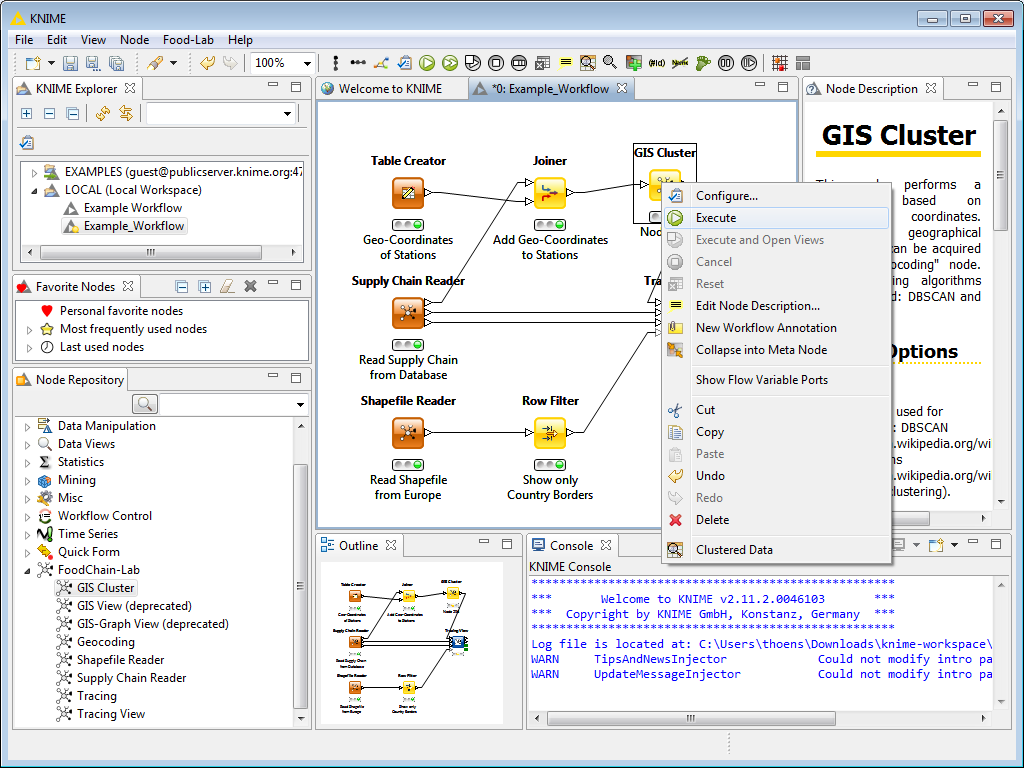
\includegraphics[width=0.9\textwidth]{8.png}
	\end{center}
	\begin{itemize}
		\item For the new condition select "type of business" as \textbf{Property} and "Primary Producer" as \textbf{Value}, since we want to cluster primary producers only.
		\item Now press \textbf{OK}.
	\end{itemize}
\end{frame}

\subsection{9}
\begin{frame}
	\begin{center}
  		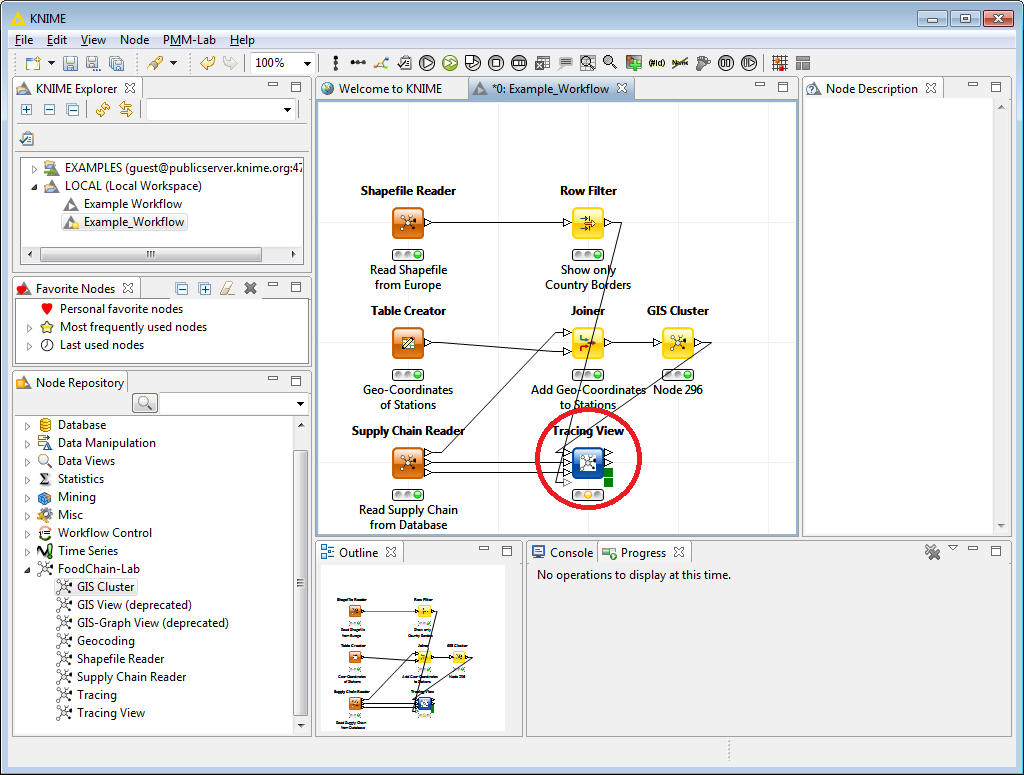
\includegraphics[height=0.6\textheight]{9.png}
	\end{center}
	\begin{itemize}
		\item Set the \textbf{Max Neighborhood Distance} to 100km. That means that stations with distance of less than 100km are put into the same cluster. For details on the algorithm look here: \url{https://en.wikipedia.org/wiki/DBSCAN}
		\item Press \textbf{OK}.
	\end{itemize}
\end{frame}

\subsection{10}
\begin{frame}
	\begin{center}
  		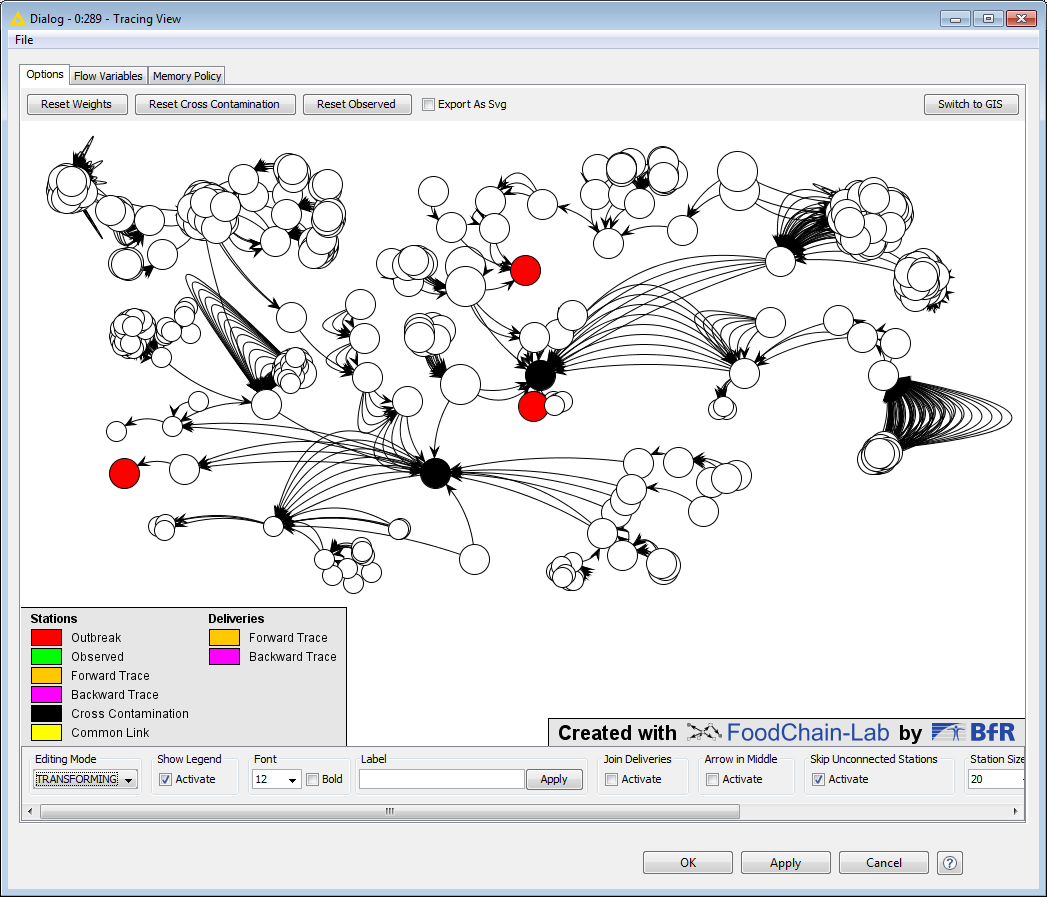
\includegraphics[height=0.6\textheight]{10.png}
	\end{center}
	\begin{itemize}
		\item Right click on \textbf{GIS Cluster} to open its context menu and select \textbf{Execute} to execute the node.
		\item The results of the clustering are put into the new column \textbf{ClusterID}. This column will now be used in the \textbf{Tracing View}.
	\end{itemize}
\end{frame}

\subsection{11}
\begin{frame}
	\begin{center}
  		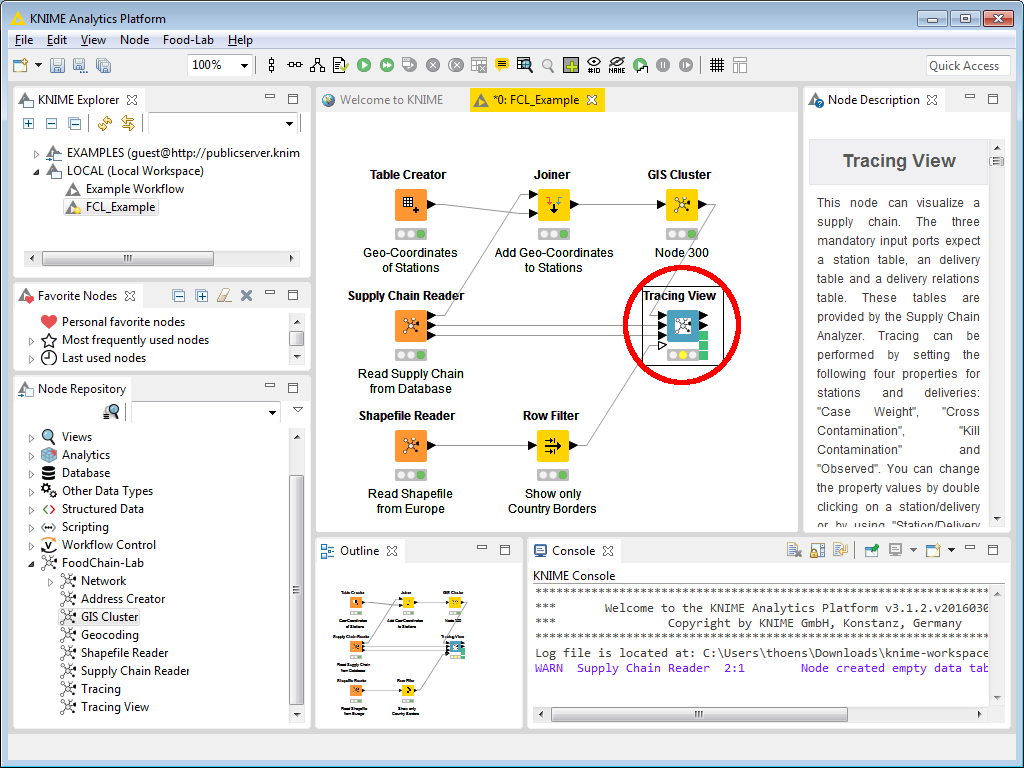
\includegraphics[height=0.6\textheight]{11.png}
	\end{center}
	\begin{itemize}
		\item Open the \textbf{Tracing View} by double-clicking on it.
	\end{itemize}
\end{frame}

\subsection{12}
\begin{frame}
	\begin{center}
  		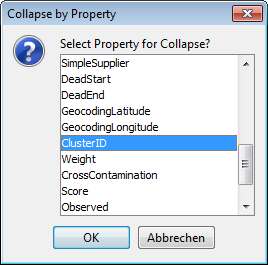
\includegraphics[height=0.6\textheight]{12.png}
	\end{center}
	\begin{itemize}
		\item A window showing the delivery network should open now.
	\end{itemize}
\end{frame}

\subsection{13}
\begin{frame}
	\begin{center}
  		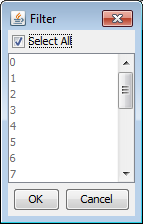
\includegraphics[height=0.6\textheight]{13.png}
	\end{center}
	\begin{itemize}
		\item Right click in the graph to open the context menu and select \textbf{Collapse by Property}.
	\end{itemize}
\end{frame}

\subsection{14}
\begin{frame}
	\begin{center}
  		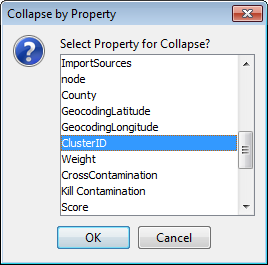
\includegraphics[height=0.5\textheight]{14.png}
	\end{center}
	\begin{itemize}
		\item The clustering will be done based on the results of the \textbf{GIS Cluster} node.
		\item Select \textbf{ClusterID} and press \textbf{OK}.
	\end{itemize}
\end{frame}

\subsection{15}
\begin{frame}
	\begin{center}
  		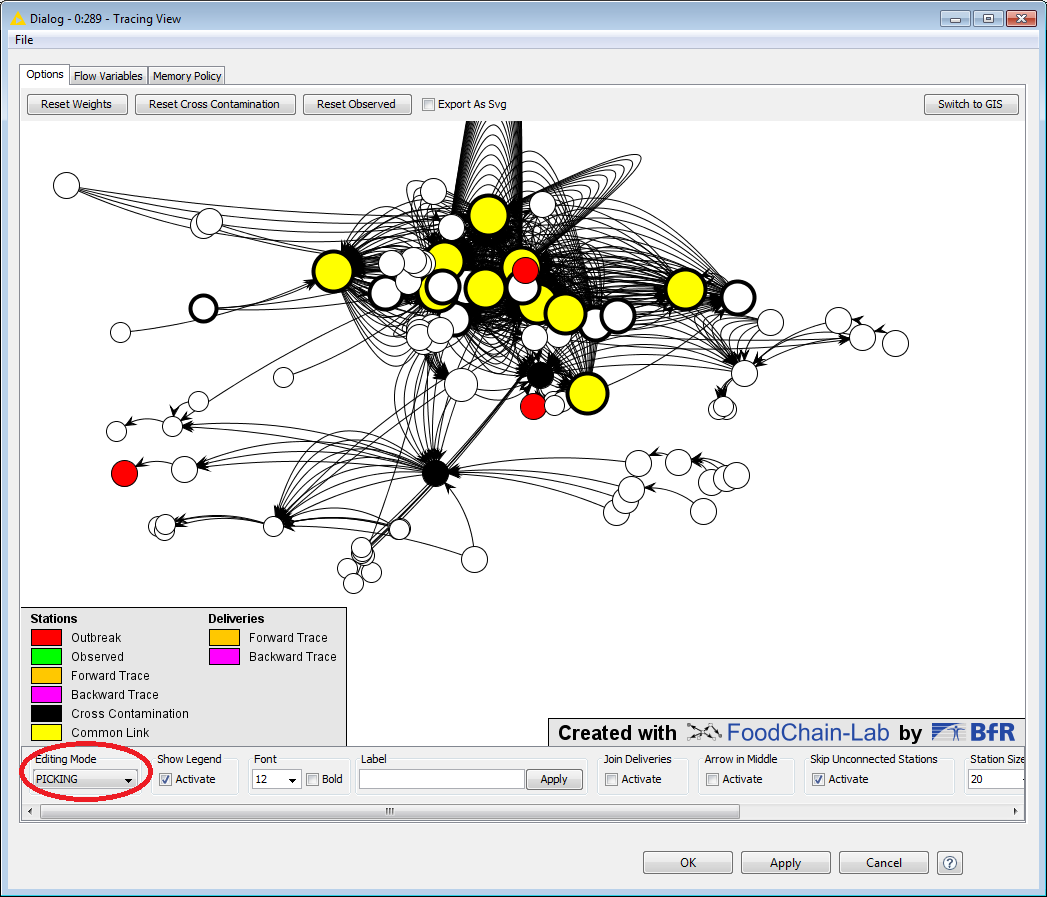
\includegraphics[height=0.5\textheight]{15.png}
	\end{center}
	\begin{itemize}
		\item Just press \textbf{OK}, since we do not want to exclude any area.
	\end{itemize}
\end{frame}

\subsection{16}
\begin{frame}
	\begin{center}
  		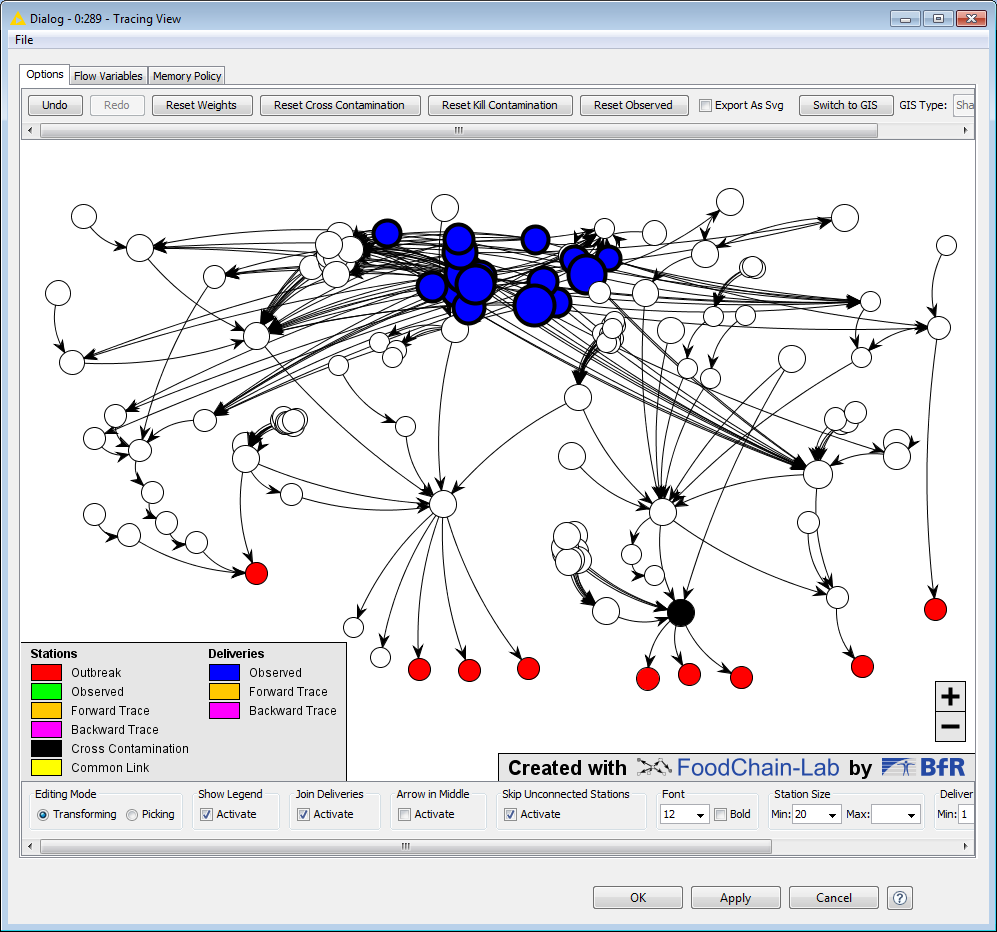
\includegraphics[height=0.6\textheight]{16.png}
	\end{center}
	\begin{itemize}
		\item All French primary producers have been clustered to areas.
		\item Each selected station (blue circle) is an area in France.		
	\end{itemize}
\end{frame}

\subsection{17}
\begin{frame}
	\begin{center}
  		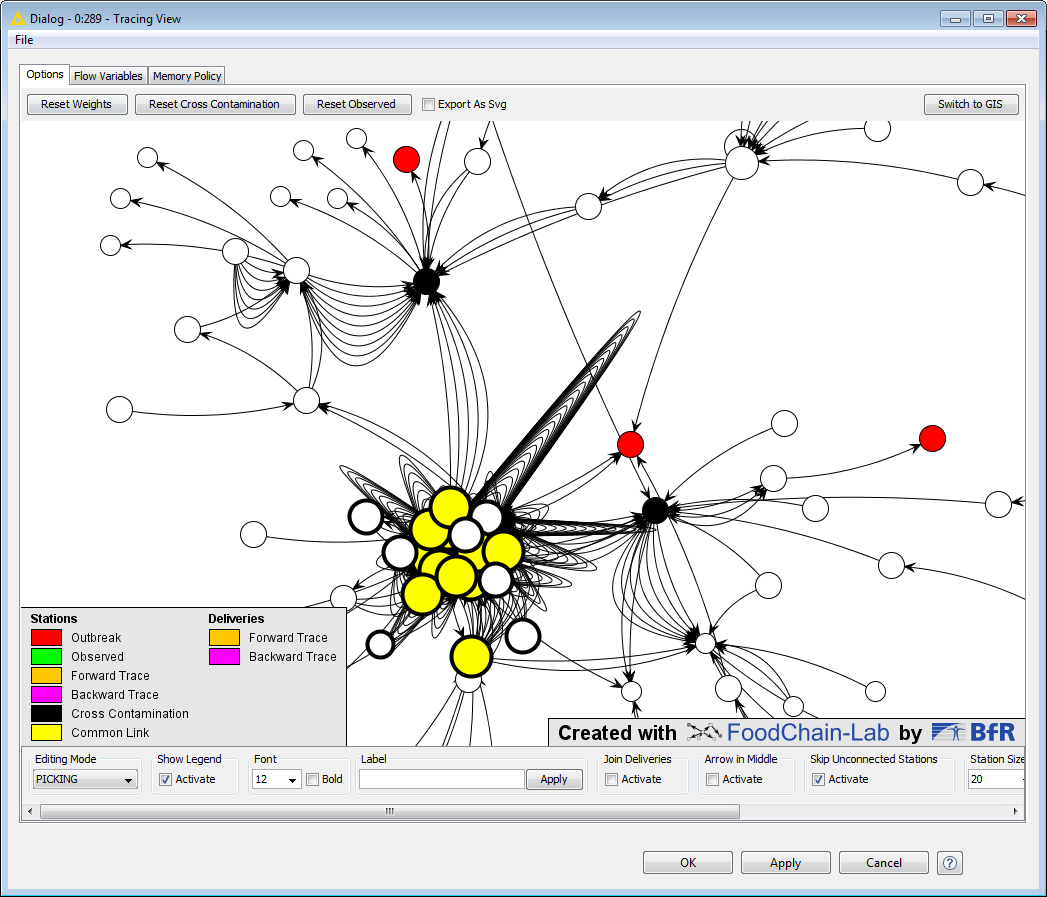
\includegraphics[height=0.6\textheight]{17.png}
	\end{center}
	\begin{itemize}
		\item Select "Picking" as \textbf{Editing Mode} and click in the graph to deselect all stations.
		\item You can now see, that one of the stations is yellow. That means, that this stations (French area) is connected to all outbreak spots (red circles).
		\item Press \textbf{Switch to GIS} to see where this area is.
	\end{itemize}
\end{frame}

\subsection{18}
\begin{frame}
	\begin{center}
  		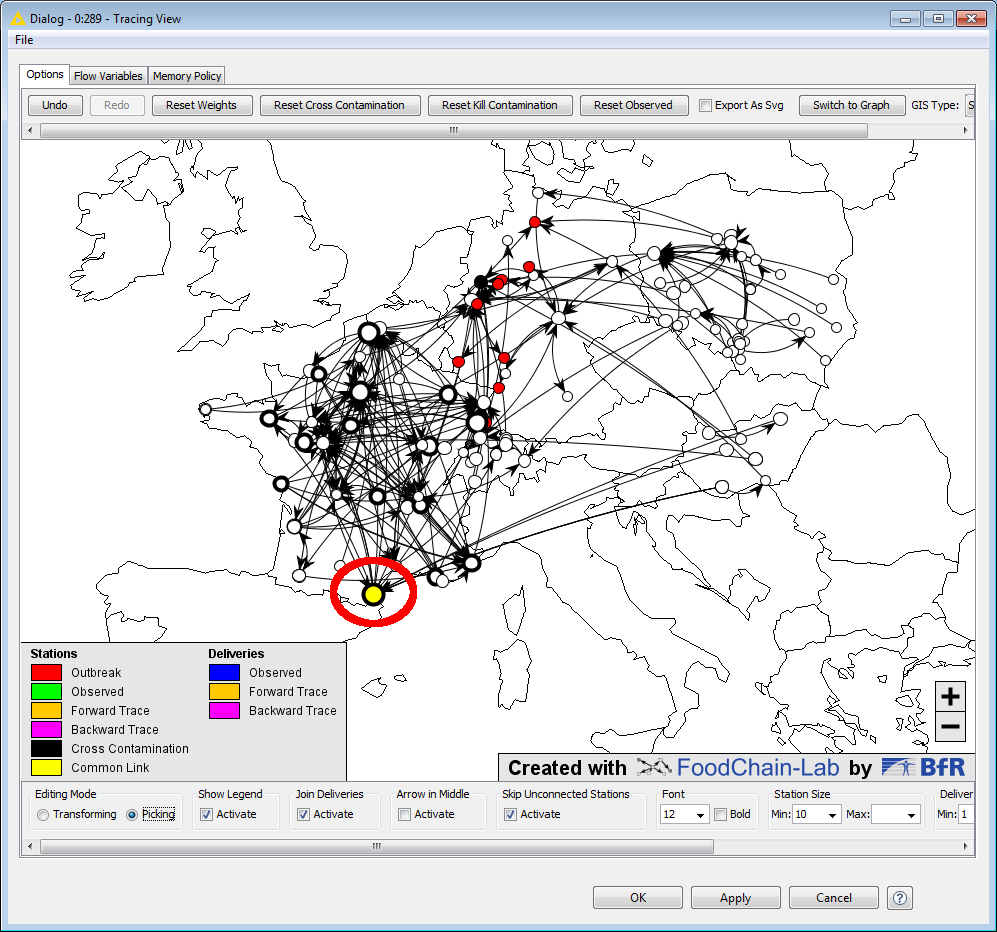
\includegraphics[height=0.6\textheight]{18.png}
	\end{center}
	\begin{itemize}
		\item The area is in Southern France.
	\end{itemize}
\end{frame}

\end{document}